% !TeX spellcheck = pl_PL
\documentclass[11pt,a4paper]{article}
\usepackage[utf8]{inputenc}
\usepackage{amsmath}
\usepackage{float}
\usepackage{amsfonts}
\usepackage{mathtools,amssymb,amsthm}
\usepackage{graphicx}
\usepackage{polski}
\mathtoolsset{showonlyrefs,mathic}
\author{Kamil Zawistowski, Michał Cerazy}


\begin{document}
\title{Pakiety statystyczne \\ Sprawozdanie 3}
\author{Michał Cerazy, Kamil Zawistowski \\ 229969, 229924}
\maketitle
\newpage
\tableofcontents
\newpage
\section{Cel}
Celem sprawozdania jest odszukanie występowania zależności między statystykami z amerykańskiej koszykówki przy użyciu modeli regresji liniowej. 

\section{Zbiór danych}
Przedmiotem badań są statystyki poszczególnych zawodników występujących na parkietach NBA w sezonie 2014/2015. Podczas tego sezonu w lidze wystąpiło 490 zawodników (każda drużyna może zatrudniać jednocześnie 15 graczy), co przekłada się na taką samą długość próbki. Polecenie wymaga co najmniej 500 pomiarów, jednak w związku z atrakcyjnością omawianych danych, zdecydowaliśmy się na ich użycie. Dane pochodzą ze strony $kaggle.com$. 
\subsection{Opis zmiennych}
Zmienne kategoryczne wyróżnione są poprzez nawiasy zawierające wartości, które zmienna może przyjąć. W sprawozdaniu zostały użyte następujące zmienne:
\begin{itemize}
	\item ,,Name'' -- imię oraz nazwisko,
	\item ,,Age'' -- wiek,
	\item ,,Birth Place'' -- miejsce urodzenia (US, NONUS),
	\item ,,Height''-- wzrost w centymetrach,
	\item ,,Pos'' -- pozycja, na której gra dany zawodnik (PG, SG, C, PF, SF),
	\item ,,Team'' -- ostatni zespół, w którym grał zawodnik,
	\item ,,Weight'' -- waga zawodnika w kilogramach,	
	\item ,,BMI'' -- wskaźnik Body Mass Index, 
	\item ,,Games Played'' - ilość rozegranych meczy w sezonie,	
	\item ,,MIN'' -- ilość minut spędzonych na boisku w sezonie,
	\item ,,PTS'' -- ilość punktów zdobytych w sezonie,
	\item ,,FGM'' -- ilość trafionych rzutów z gry w sezonie,
	\item ,,FGA'' -- ilość rzutów z gry w sezonie,
	\item ,,FGp'' -- procentowa skuteczność rzutów z gry w sezonie,
	\item ,,ThreePM'' -- ilość trafionych rzutów za 3 punkty w sezonie,
	\item ,,ThreePA'' -- ilość rzutów za 3 punkty w sezonie,
	\item ,,ThreePp'' -- procentowa skuteczność rzutów za trzy punkty w sezonie,
	\item ,,FTM'' -- ilość trafionych rzutów osobistych w sezonie,
	\item ,,FTA'' -- ilość rzutów osobistych w sezonie,
	\item ,,FTp'' -- procentowa skuteczność rzutów osobistych w sezonie,
	\item ,,OREB'' -- ilość zbiórek ofensywnych w sezonie,	
	\item ,,DREB'' -- ilość zbiórek defensywnych w sezonie,	
	\item ,,REB'' -- ilość zbiórek w sezonie,
	\item ,,AST'' -- ilość asyst w sezonie,
	\item ,,STL'' -- ilość przechwytów w sezonie,
	\item ,,BLK'' -- ilość bloków w sezonie,
	\item ,,TOV'' -- ilość strat w sezonie,
	\item ,,PF'' -- ilość fauli osobistych w sezonie,
	\item ,,EFF'' -- wydajność zawodnika,
	\item ,,AST/TOV'' -- stosunek ilości asyst do ilości strat,
	\item ,,STL/TOV'' -- stosunek ilości przechwytów do ilości strat.
\end{itemize}
	Dodatkowo, na potrzeby modeli wprowadziliśmy dodatkowe kolumny takie jak:
\begin{itemize}	
	\item ,,PPG'' -- średnia ilość punktów zdobywanych na mecz,
	\item ,,MPG'' -- średnia ilość minut rozegranych na mecz,
	\item ,,FTAPG'' -- średnia ilość rzutów osobistych na mecz,
	\item ,,FGAPG'' -- średnia ilość rzutów z pola na mecz,
	\item ,,ThreeAPG'' -- średnia ilość rzutów za 3 punkty na mecz.
\end{itemize}
%\subsection{Wybór zmiennych zależnych i niezależnych}
%	Jako zmienną zależną będziemy rozważać średnią ilość punktów zdobywanych na mecz. Do zmiennych niezależnych należą !!!! UZUPEŁNIĆ ZMIENNE NIEZALEŻNE !!!!. Decydujemy się na taki wybór, gdyż chcemy poznać wpływ poszczególnych statystyk na liczbę zdobywanych punktów. (?) Odnalezienie odpowiedniego modelu będzie podstawą do wyznaczania zawodników pretendujących do bycia najlepiej punktującymi w kolejnych sezonach. (?)
	
\section{Dopasowanie modelu}
Jako zmienną zależną będziemy rozważać średnią ilość punktów zdobywanych na mecz. Zasugerowane przez nas modele będą się różnić doborem zmiennych niezależnych, jednakże w każdym z nich używać będziemy średniej ilości rozegranych minut na mecz, gdyż jest to niezbędna informacja do analizy modelu. Dodatkowo, w naszych rozważaniach korzystać będziemy z cech fizycznych zawodników, statystyk rzutowych, pochodzenia i pozycji, dlatego usuniemy dane dotyczące asyst, bloków, zbiórek, przechwytów, strat oraz drużyn, w których skończyli sezon.

\subsection{Poprawność modeli}
Na wstępie należy zaznaczyć, że żaden z naszych modeli nie spełnia warunku normalności residuów. Pomimo wielu podjętych prób nie udało nam się przekształcić danych tak, by residua modelu pochodziły z rozkładu normalnego. Normalizacji residuów próbowaliśmy dokonać poprzez:
\begin{itemize}
	\item nałożenie logarytmu na zmienną zależną,
	\item nałożenie pierwiastków na zmienną zależną,
	\item nałożenie potęgi na zmienną zależną,
	\item usuwanie wartości odstających,
	\item usuwanie wartości o dużej dźwigni.
\end{itemize}
Dodatkowo, w każdy zaproponowany przez nas model nie posiada stałej, gdyż po sprawdzeniu kilku możliwości zauważyliśmy, że modele bez niej charakteryzują się lepszym dopasowaniem.
\subsection{Model I: umiejętności rzutowe zawodników}
Przy pierwszym ze sprawdzanych przez nas modeli skupimy się na zdolnościach rzutowych, a więc zmiennymi objaśniającymi będą średnia ilość rzutów z pola, skuteczność z pola, średnia ilość rzutów za 3 punkty, skuteczność rzutów za 3 punkty, średnia ilość rzutów osobistych, skuteczność rzutów osobistych oraz średnia ilość minut przegranych w meczu. W tabeli \ref{offense} przedstawione zostały wartości współczynników oraz pozostałe statystyki dla omawianego modelu. 

\begin{table}[H]
	\begin{center}
	\begin{tabular}{| c | c | c | c | c |}
		\hline
		Zmienna & Estymacja & Błąd standardowy & T-wartość & Pr$(<|t|)$\\ \hline
		FGAPG & 0.961931 & 0.025304 & 38.015 & $<$2e-16\\ \hline
		FGp & 0.012008 & 0.003441 & 3.490 & 0.000528\\ \hline
		ThreeAPG & 0.130223 & 0.032714 & 3.981 & 7.93e-05\\ \hline 
		ThreePp & 0.001808 & 0.002931 & 0.617 & 0.537764\\ \hline
		FTAPG & 0.842080 & 0.044256 & 19.027 & $<$2e-16\\ \hline
		FTp  & -0.007247 & 0.002059 & -3.519 & 0.000474\\ \hline
	\end{tabular}
	\caption{Model rzutowy - współczynniki modelu}
	\label{offense}
	\end{center}
\end{table}

\begin{figure}[t]
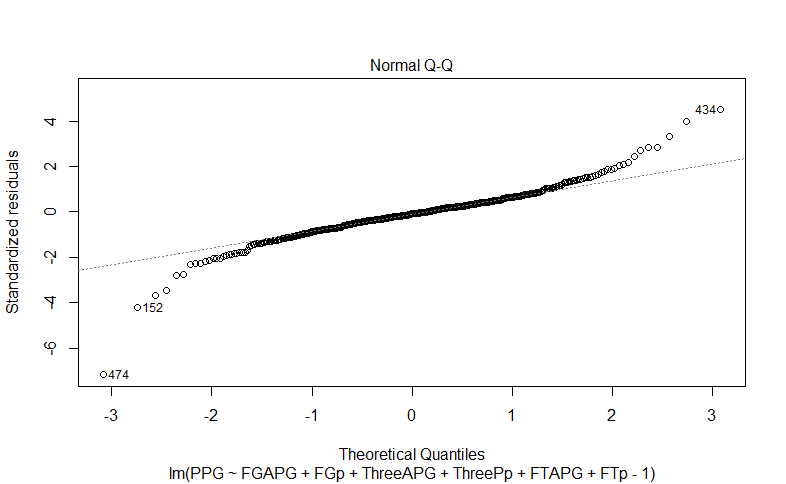
\includegraphics[width=\textwidth]{offense_2}
\caption{QQplot dla modelu rzutowego}
\label{qqplot_offense}
\centering
\end{figure}
Jak można zauważyć, wszystkie parametry poza skutecznością rzutów za 3 punkty są istotne( co może dziwić przy obecnych realiach gry w koszykówkę, gdzie coraz większą wagę przykłada się do szybkich rzutów trzypunktowych). Jak się okazało, w przypadku tego modelu założenia nie są spełnione: test Shapiro-Wilka i spojrzenie na Rysunek \ref{qqplot_offense} odrzuciły hipotezę o normalności residuów, a testy badające średnią i wariancję( polegające na wielokrotnym losowaniu próbki 50 elementów i przeprowadzaniu t.testu i var.testu) wykazały, że średnia jest różna od zera oraz wariancja nie jest stała na poziomie istotności $\alpha=0.05$. Wyniki zawarte zostały w Tabeli \ref{zalozenia_offense}.
\begin{table}[H]
	\begin{center}
	\begin{tabular}{| c | c | c | c |}
		\hline
		W & p-value & ConstMeanMC & ConstVarMC\\ \hline
		0.92953 & 2.028e-14 & 0.1019 & 0.2892 \\ \hline
	\end{tabular}
	\caption{Model rzutowy - testy założeń}
	\label{zalozenia_offense}
	\end{center}
\end{table}
\begin{figure}[t]
	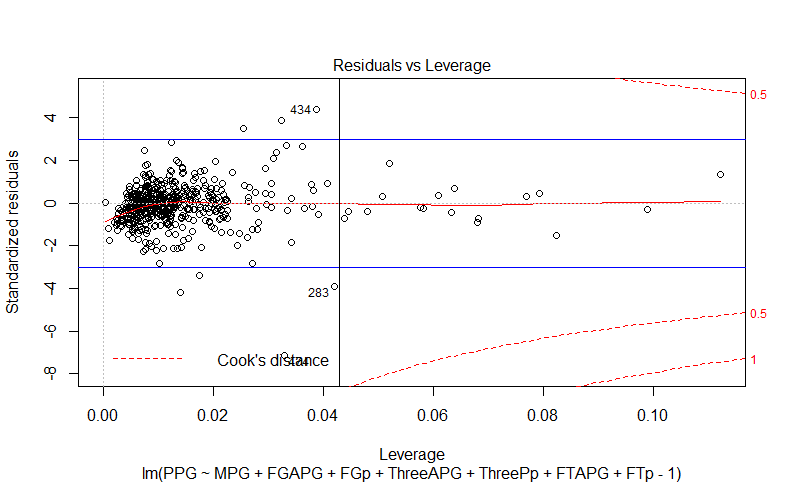
\includegraphics[width=\textwidth]{offense_4}
	\caption{Wykres residuów i dźwigni dla modelu rzutowego}
	\label{leverage_offense}
	\centering
\end{figure}
Na Rysunku \ref{leverage_offense} niebieskimi liniami zaznaczono próg dla wartości odstających, czarną natomiast tych o wysokiej dźwigni. Niestety, po ich usunięciu model nadal nie spełniał założeń i pojawiły się kolejne problematyczne obserwacje( próbowaliśmy eliminować je do skutku, jednak również to nie przyniosło oczekiwanych rezultatów).
\subsection{Model II: pozycje zawodników}
Podczas tworzenia tego modelu staraliśmy się określić, czy pozycja zawodnika wpływa na ilość zdobywanych przez niego punktów, dlatego jako zmienne objaśniające przyjęliśmy pozycję danego gracza, średnią ilość czasu spędzanego na boisku oraz jego wiek. W tabeli \ref{position} przedstawione są współczynniki dopasowanego modelu. Jak widać, wszystkie zmienne poza wiekiem okazały się być istotne. 
\begin{table}[H]
	\begin{center}
		\begin{tabular}{| c | c | c | c | c |}
			\hline
			Zmienna & Estymacja & Błąd standardowy & T-wartość & Pr$(<|t|)$\\ \hline
			PosC & -2.654071 &  0.807253 & -3.288 & 0.001084 \\ \hline
			PosPF &-2.535002 &  0.793808 & -3.193 & 0.001498 \\ \hline
			PosPG &-2.506314 &  0.799289 & -3.136 &  0.001819 \\ \hline
			PosSF &-3.007021 &  0.810325 & -3.711 & 0.000231\\ \hline
			PosSG &-2.355508 &  0.782667 & -3.010 & 0.002753 \\ \hline
			MPG   & 0.542043 &  0.012523 & 43.282 & $< 2e-16$\\ \hline
			Age   &-0.008325 &  0.026757 & -0.311 & 0.755835 \\ \hline
		\end{tabular}
		\caption{Model pozycyjny - współczynniki modelu}
		\label{position}
	\end{center}
\end{table}
W tabeli \ref{zalozenia_position} przedstawione są wyniki testu Shapiro-Wilka oraz testów średniej i wariancji residuów. Jak wyżej wspomnieliśmy, model nie spełnia założenia normalności badanych wartości resztowych( jak widać również na Rysunku \ref{qqplot_position}). Na Rysunku \ref{leverage_position} zaznaczone zostały wartości odstające, których usunięcie również nie pomogło w normalizacji residuów.
\begin{table}[H]
	\begin{center}
		\begin{tabular}{| c | c | c | c |}
			\hline
			W & p-value & ConstMeanMC & ConstVarMC\\ \hline
			0.95198 & 1.644e-11 & 0.0424 & 0.1784 \\ \hline
		\end{tabular}
		\caption{Model pozycyjny - testy założeń}
		\label{zalozenia_position}
	\end{center}
\end{table}
\begin{figure}[t]
	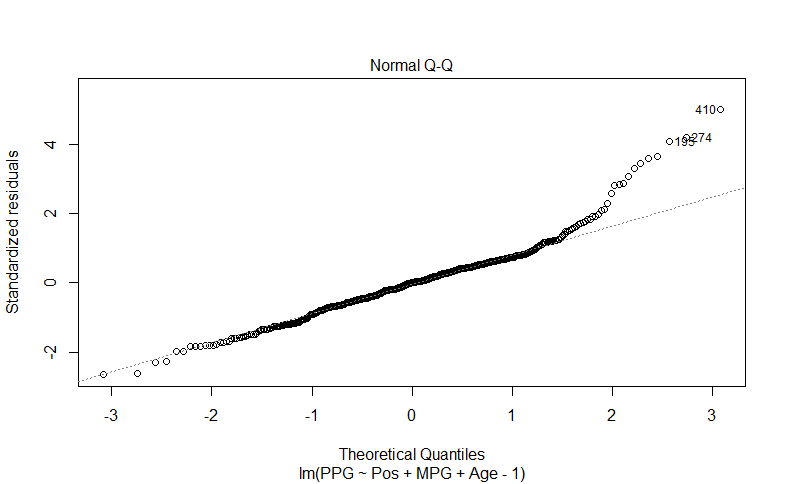
\includegraphics[width=\textwidth]{position_2}
	\caption{QQplot dla modelu uwzględniającego pozycje}
	\label{qqplot_position}
	\centering
\end{figure}
\begin{figure}[t]
	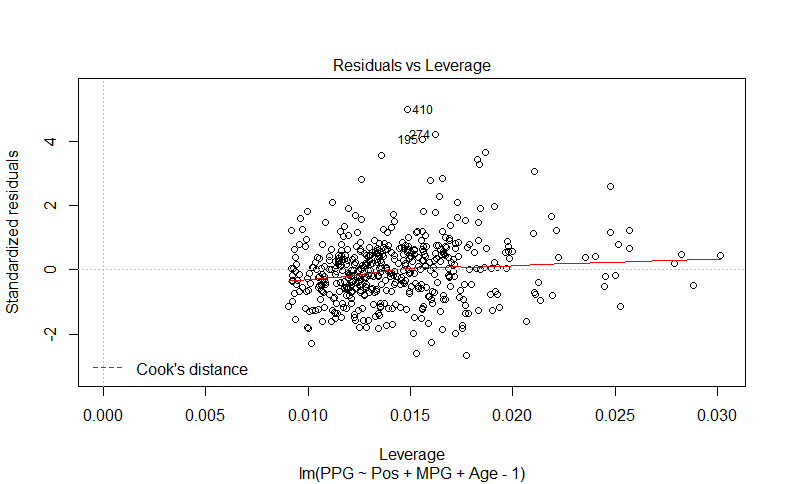
\includegraphics[width=\textwidth]{position_4}
	\caption{Wykres residuów i dźwigni dla modelu uwzględniającego pozycje}
	\label{leverage_position}
	\centering
\end{figure}

\subsection{Model III: pochodzenie zawodników}
Przy ostatnim z badanych modeli chcieliśmy zbadać, czy zawodnicy ze Stanów Zjednoczonych, stanowiący większość ligi, są lepszymi punktującymi niż obcokrajowcy.
Jako zmienne objaśniające przyjęliśmy średnią ilość minut na mecz oraz pochodzenie zawodnika. W Tabeli \ref{origin} przedstawione są współczynniki dobranego modelu, gdzie jak można zauważyć, wszystkie parametry poza iloczynem średniej ilości minut na mecz i indykatora urodzenia w USA okazały się być istotnymi.
Testy badające średnią i wariancję wykazały, że średnia jest różna od zera oraz wariancja nie jest stała na poziomie istotności $\alpha=0.05$. Wyniki zawarte zostały w Tabeli \ref{zalozenia_offense}.
\begin{table}[H]
	\begin{center}
		\begin{tabular}{| c | c | c | c |}
			\hline
			W & p-value & ConstMeanMC & ConstVarMC\\ \hline
			0.95802 & 1.347e-10 & 0.0416 & 0.1664 \\ \hline
		\end{tabular}
		\caption{Model rzutowy - testy założeń}
		\label{zalozenia_origin}
	\end{center}
\end{table}
\begin{table}[H]
	\begin{center}
		\begin{tabular}{| c | c | c | c | c |}
			\hline
			Zmienna & Estymacja & Błąd standardowy & T-wartość & Pr$(<|t|)$\\ \hline
			MPG    &            0.49746  &  0.02803 & 17.746 & $< 2e-16$\\ \hline
			Birth Placenon us & -2.05640 &   0.60703&  -3.388 & 0.000762 \\ \hline
			Birth Placeus   &  -3.02104  &  0.30683 & -9.846  & $< 2e-16$ \\ \hline
			MPG:Birth Placeus & 0.05583  &  0.03123 &  1.788 & 0.074431 \\ \hline
		\end{tabular}
		\caption{Model uwzględniający pochodzenie - współczynniki modelu}
		\label{origin}
	\end{center}
\end{table}
Na Rysunku \ref{qqplot_origin} przedstawiony jest wykres kwantyl--kwantyl, którego ocena utwierdza nas w przekonaniu, że residua nie pochodzą z rozkładu normalnego.
\begin{figure}[t]
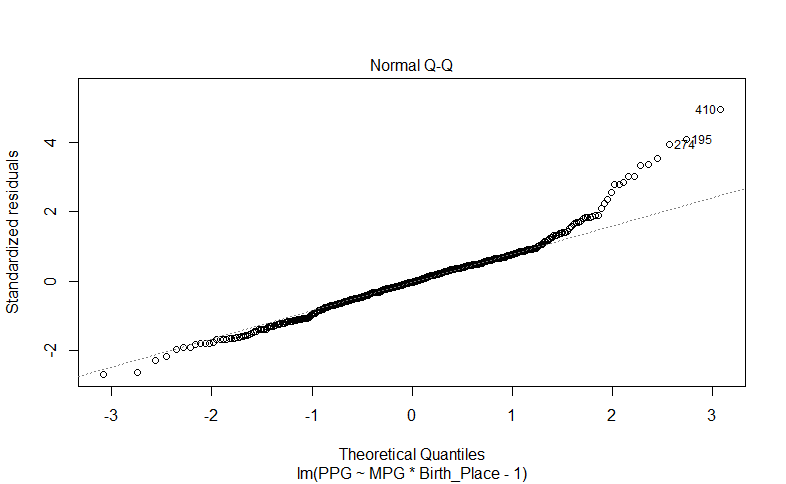
\includegraphics[width=\textwidth]{origin_2}
\caption{QQplot dla modelu uwzględniającego pochodzenie}
\label{qqplot_origin}
\centering
\end{figure}
Rysunek \ref{leverage_origin} przedstawia wartości odstające oraz o dużej dźwigni, których usunięcie również nie wpłynęło pozytywnie na poprawność modelu.
\begin{figure}[t]
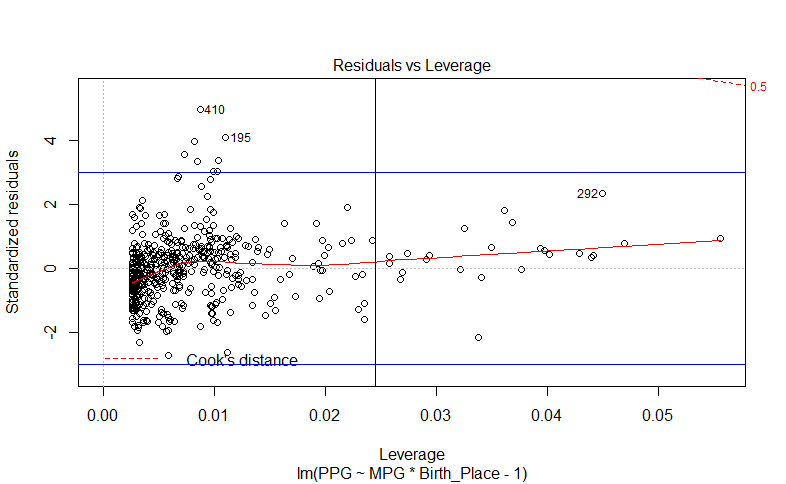
\includegraphics[width=\textwidth]{origin_4}
\caption{Wykres residuów i dźwigni dla modelu uwzględniającego pochodzenie}
\label{leverage_origin}
\centering
\end{figure}

\subsection{Porównanie modeli}
Znając współczynniki dobranych modeli wyznaczyliśmy:
\begin{itemize}
	\item współczynnik determinacji, oznaczany jako $R^2$.
	\item skorygowany współczynnik determinacji, oznaczany jako $aR^2$,
	\item kryterium Akaikego, oznaczane jako $AIC$,
	\item logarytm wskaźnika wiarygodności, oznaczany jako $LogLik$.
\end{itemize}

\begin{table}[H]
	\begin{center}
		\begin{tabular}{| c | c | c | c | c |}
			\hline
			Model & $R^2$ & $aR^2$ & AIC & LogLik \\ \hline
			I & 0.99317 & 0.993 & 1204.576 & -594.288\\ \hline
			II & 0.9374 & 0.9365 & 2283.041 & -1133.52\\ \hline 
			III & 0.9375 & 0.937 & 2281.154 & -1135.577\\ \hline  
		\end{tabular}
		\caption{Porównanie modeli}
		\label{porownanie_modeli}
	\end{center}
\end{table}
Podsumowując wyżej wymienione modele można stwierdzić, że najlepszym z nich jest model uwzględniający umiejętności rzutowe zawodników. Taki wniosek nasuwa się po analizie Tabeli \ref{porownanie_modeli}. Współczynniki determinacji oraz logarytm wskaźnika wiarygodności są największe dla tego właśnie modelu, co oznacza, że jest on najlepiej dopasowany do naszych danych. Taką konkluzję potwierdza również kryterium informacyjne Akaikego, które najmniejszą wartość przyjmuje dla modelu nr I.

\section{Inne testowane modele}
\subsection{Model uwzględniający cechy motoryczne zawodników}
Podjęliśmy trzy próby dobrania najlepszego modelu, który uzależniony jest od predyspozycji fizycznych zawodników. Oczywiście, każdy z tych modeli musi być rozszerzony o ilość rozegranych minut na mecz, gdyż jest to niezbędna informacja do analizy modelu.

\subsubsection{Model WWW}
Pierwszy z dopasowywanych modeli uwzględnia wzrost, wiek oraz wagę zawodników. Wpływową zmienną okazała się być ilość minut na mecz (jak zakładaliśmy wyżej, jest to najważniejszy czynnik) oraz waga zawodnika. W tabeli \ref{model_www} przedstawione zostały wartości współczynników oraz pozostałe statystyki dla omawianego modelu. 
\begin{table}[H]
	\begin{tabular}{| c | c | c | c | c |}
		\hline
		Zmienna & Estymacja & Błąd standardowy & T-wartość & Pr$(<|t|)$\\ \hline
		Stała & 1.55894  &  3.46942&   0.449&   0.6534    \\ \hline
		Wzrost &     -0.03357 &   0.02288 & -1.467  & 0.1430    \\ \hline
		Minuty na mecz &         0.54145  &  0.01245&  43.474  &$ <2e-16$\\ \hline
		Waga  &     0.02764    &0.01643 &  1.683  & 0.0931  \\ \hline
		Wiek   &      -0.01751  &  0.02678 & -0.654&   0.5136 \\ \hline
	\end{tabular}
	\caption{Model WWW - współczynniki modelu}
	\label{model_www}
\end{table}
\subsubsection{Model WW}
Drugi z dopasowywanych modeli uwzględnia średni czas gry, wzrost oraz wagę zawodników. Odjęcie wieku ma na celu sprawdzenie jak zachowa się model po odjęciu jednej zmiennej nie będącej zmienną istotną. W tabeli \ref{model_ww} przedstawione zostały współczynniki modelu WW. Jak można zauważyć zmienne istotne dla nie zmieniły się, jednakże waga jest na granicy zostania zmienną istotną.

\begin{table}[H]
	\begin{tabular}{| c | c | c | c | c |}
		\hline
		Zmienna & Estymacja & Błąd standardowy & T-wartość & Pr$(<|t|)$\\ \hline
		Minuty na mecz & 0.541663 & 0.012207 & 44.372 & $<$2e-16\\ \hline
		Wzrost & -0.026028 & 0.006499 & -4.005 & 7.17e-05 \\ \hline 
		Waga & 0.023444 & 0.012429 & 1.886 & 0.0599 \\ \hline
	\end{tabular}
	\caption{Model WW - współczynniki modelu}
	\label{model_ww}
\end{table}

\subsubsection{Model WB}
Trzeci z dopasowywanych modeli uwzględnia wiek oraz wskaźnik BMI. Omawiany wskaźnik jest popularną statystyką mówiącą o stanie zdrowia fizycznego i wyliczana jest na podstawie poniższego wzoru:
\begin{equation}
BMI = \frac{waga}{wzrost^2}.
\end{equation}
W związku z tym niejawnie do modelu włączamy wagę i wzrost zawodników ligi. Wyniki tego zabiegu przedstawione są w tabeli \ref{model_wb}. Ponownie, wiek okazał się być nieistotny, natomiast BMI oraz ilość minut na mecz są istotne.
\begin{table}[H]
	\begin{tabular}{| c | c | c | c | c |}
		\hline
		Zmienna & Estymacja & Błąd standardowy & T-wartość & Pr$(<|t|)$\\ \hline
		Minuty na mecz & 0.53943 & 0.01245 & 43.329 & $<$2e-16\\ \hline
		Wiek & -0.03886 & 0.02571 & -1.512 & 0.1313\\ \hline 
		BMI & -0.06666 & 0.02896 & -2.302 &  0.0218\\ \hline 	
	\end{tabular}
	\caption{Model WB - współczynniki modelu}
	\label{model_wb}
\end{table}
\subsection{Porównanie modeli}
W tabeli \ref{porownanie_modeli_w} widać, że model WB cechuje się najlepszym dopasowaniem do danych według współczynnika $R^2$. Kryterium informacyjne Akaikego przemawia za wybraniem drugiego modelu jako najlepiej opisującego badany zbiór wartości. Logarytm wskaźnika wiarygodności wskazuje z kolei na model WWW. Korzystając z metody analizy wariancji ustaliliśmy, że model WB jest modelem istotnym spośród wszystkich modeli W. Należy jednak zaznaczyć, że żaden z modeli nie spełnia założenia normalności residuów, mimo wielu prób manipulacji danymi.
\begin{table}[h]
	\begin{center}
		\begin{tabular}{| c | c | c | c |}
			\hline
			Model & $R^2$ & AIC & LogLik\\ \hline
			WWW & 0.7974 & 2283.606 & -1135.803\\ \hline
			WW & 0.9358  & 2280.111 & -1136.055 \\ \hline 
			WB & 0.937 & 2288.041 & -1140.021 \\ \hline  
		\end{tabular}
		\caption{Porównanie modeli}
		\label{porownanie_modeli_w}
	\end{center}
\end{table}

\section{Podsumowanie}
W naszym sprawozdaniu dobraliśmy kilka modeli opisujących zdobywanie punktów przez koszykarzy w zależności od wielu czynników. Model opisujący zdolności rzutowe okazał się być istotnie najlepszym spośród wszystkich testowanych, na co wskazywały wyznaczone przez nas statystyki. Niestety, pomimo starań, nie udało nam się znaleźć (lub doprowadzić do) modelu spełniającego założenia.
\end{document}